\documentclass[compress,aspectratio=43]{beamer}
% beamer-setup.tex
% 2024-09-21

\usetheme{default}
\usecolortheme{default}
\useoutertheme[subsection=false]{miniframes}
\usefonttheme[onlymath]{serif}

\definecolor{simplebeamercolor}{RGB}{57,89,199}
\setbeamercolor{structure}{fg=simplebeamercolor} % default color: rgb{0.2 0.2 0.7}

\setbeamertemplate{footline}[frame number]{}
\setbeamertemplate{navigation symbols}{}

\setbeamercolor{section in head/foot}{fg=white, bg=structure}

\setbeamertemplate{title page}[default][colsep=-4bp,rounded=true,shadow=true]
\setbeamercolor*{title}{use=structure,fg=white,bg=structure.fg}

\setbeamertemplate{section in toc}[sections numbered]
\setbeamertemplate{subsection in toc}[subsections numbered]

\setbeamerfont{institute}{size=\normalsize}
\setbeamerfont{footnote}{size=\tiny}

\setbeamercolor{block body}{bg=structure!10}
\setbeamercolor{block title}{bg=structure!20}
\setbeamercolor{block body alerted}{bg=alerted text.fg!10}
\setbeamercolor{block title alerted}{bg=alerted text.fg!20}
\setbeamercolor{block body example}{bg=green!10}
\setbeamercolor{block title example}{bg=green!20}
\setbeamercolor{block title proof}{bg=white}
\setbeamercolor{block body proof}{bg=white}

\setbeamertemplate{itemize items}[circle]
\setbeamertemplate{enumerate items}[default]

\setbeamertemplate{caption}[numbered]

\AtBeginSection[]
{
    \begin{frame}<beamer>{Outline}
        \tableofcontents[currentsection,currentsubsection,
            hideothersubsections,sectionstyle=show/shaded]
    \end{frame}
}

% fonts
\usepackage[T1]{fontenc}
% \usepackage{palatino}
\usepackage{mathrsfs}
\usepackage{calligra}
\usepackage{bm}

% math
\usepackage{amsmath,amsthm,amsfonts,amssymb}

\usepackage{extarrows}
\usepackage{booktabs}
\usepackage{multirow}
\usepackage{multicol}
\usepackage{subcaption}

\usepackage{hyperref}
\hypersetup{
    colorlinks=true,
    linkcolor=,
    filecolor=blue,
    urlcolor=blue,
    citecolor=cyan,
}

\usepackage{graphicx}
\graphicspath{
    {./figure/}{./figures/}{./image/}{./images/}{./graphic/}{./graphics/}{./picture/}{./pictures/}
}

\usepackage[ruled,linesnumbered,noline]{algorithm2e}

\usepackage{listings}
\lstdefinestyle{mystyle}{
    basicstyle=\small\ttfamily,
    commentstyle=\color[RGB]{34,139,34},
    keywordstyle=\color[RGB]{0,0,255},
    numberstyle=\tiny\color{gray},
    stringstyle=\color[RGB]{128,0,128},
    identifierstyle=\color{black},
    showstringspaces=false,
    tabsize=4,
    breaklines=true,
    numbers=left,
    frame=single,
    rulecolor=\color{black},
    captionpos=b,
    xleftmargin=\parindent,
    aboveskip=\baselineskip,
    belowskip=\baselineskip,
    escapeinside={\%*}{*)},
}
\lstset{style=mystyle}


\usepackage[style=authoryear]{biblatex}
\addbibresource{reference.bib}

\title{Title}
\subtitle{Subtitle}
\author{Author}
\date{\today}
\institute{University of XXXX}

\AtBeginSection[]{
    \begin{frame}<beamer>{Outline}
        \tableofcontents[currentsection,currentsubsection]
    \end{frame}
}
\AtBeginSubsection[]{
    \begin{frame}<beamer>{Outline}
        \tableofcontents[currentsection,currentsubsection]
    \end{frame}
}

\begin{document}

\begin{frame}[plain]
    \titlepage
\end{frame}

\begin{frame}{Outline}
    \tableofcontents
\end{frame}

\section{Guide}

\begin{frame}{Global Structure}
    To create the ``global structure" of a presentation, with the time constraints in mind, proceed as follows:

    \medskip
    \begin{enumerate}
        \item Make a mental inventory of the things you can reasonably talk about within the time available.

        \item Categorize the inventory into sections and subsections. Both the sections and the subsections should follow a logical pattern.

        \item Do not use more than four sections and not less than two per part.

        \item Keep section and subsection titles self-explaining.
    \end{enumerate}

\end{frame}

\begin{frame}{Time Control}
    \begin{itemize}
        \item A simple rule for the number of frames is that you should have at most one frame per minute.

              \medskip
        \item In most situations, you will have less time for your presentation than you would like.

              \medskip
        \item Do not try to squeeze more into a presentation than time allows for.
    \end{itemize}
\end{frame}


\begin{frame}{Beginning and End}
    People pay most attention at the beginning and at the end of talks.

    \medskip
    \begin{itemize}
        \item Begin with an explanation of what your talk is all about. Then explain what you or someone else has found out concerning the subject matter.

              \medskip
        \item Always conclude your talk with a summary that repeats the main message of the talk in a short and simple way.
    \end{itemize}

\end{frame}

\begin{frame}{Frame Title}
    \begin{enumerate}
        \item The title should really explain things, not just give a cryptic summary that cannot be understood unless one has understood the whole slide.

              \medskip
        \item In English, you should either always capitalize all words in a frame title except for words like ``a" or ``the" (as in a title), or you always use the normal lowercase letters.
              \begin{itemize}
                  \item Introduction to Algorithms.
                  \item Introduction to algorithms.
              \end{itemize}
    \end{enumerate}
\end{frame}

\begin{frame}{Frame Content}
    \begin{enumerate}
        \item Use block environments like `theorem' and so on.

              \medskip
        \item Prefer enumerations and itemize environments over plain text.

              \medskip
        \item Do not use more than two levels of subitemizing.

              \medskip
        \item A frame with too little on it is better than a frame with too much on it.
    \end{enumerate}
\end{frame}

\begin{frame}{Graphic}
    \begin{enumerate}
        \item Visualization is helpful to the audience.

              \medskip
        \item Like text, you should explain everything that is shown on a graphic.

              \medskip
        \item Sometimes the complexity of a graphic is intentional and you are willing to spend much time explaining the graphic in great detail.
    \end{enumerate}

\end{frame}

\section{Demo}

\subsection{Basic}

\begin{frame}{Highlighted Math}
    Some important formulas will be \alert{highlighted} because it's important.

    \medskip
    We consider the system of linear equations
    \begin{equation}\label{eq:LE}
        \tcbhighmath{Ax = b}
    \end{equation}
    where $A\in\mathbb{R}^{n \times n}$, $b\in\mathbb{R}^n$.
\end{frame}

\begin{frame}{Reference}
    Dynamical Low-Rank Approximation \footfullcite{kochDynamicalLowRank2007}.
\end{frame}

\begin{frame}{Columns \& Description \& List}

    \begin{columns}

        \begin{column}{0.49\textwidth}
            \begin{description}
                \item[Description 1] Explanation 1
                \item[Description 2] Explanation 2
                \item[Description 3] Explanation 3
            \end{description}
        \end{column}

        \hfill

        \begin{column}{0.49\textwidth}
            \begin{itemize}
                \item Item 1
                \item Item 2
                      \begin{enumerate}
                          \item First item
                          \item Second item
                          \item Third item
                      \end{enumerate}
                \item Item 3
                      \begin{enumerate}
                          \item First item
                          \item Second item
                      \end{enumerate}
            \end{itemize}
        \end{column}
    \end{columns}

\end{frame}

\subsection{Block}

\begin{frame}
    \frametitle{Blocks 1}
    \begin{block}{Block Title}
        This is a regular block.
    \end{block}

    \begin{alertblock}{Alert Block Title}
        This is an alert block.
    \end{alertblock}

    \begin{exampleblock}{Example Block Title}
        This is an example block.
    \end{exampleblock}
\end{frame}

\begin{frame}
    \frametitle{Blocks 2}
    \begin{definition}[XXX]
        This is a definition block.
    \end{definition}

    \begin{lemma}[XXX]
        This is a lemma block.
    \end{lemma}

    \begin{corollary}[XXX]
        This is a corollary block.
    \end{corollary}

    \begin{example}[XXX]
        This is an example block.
    \end{example}

\end{frame}

\begin{frame}
    \frametitle{Blocks 3}
    \begin{theorem}[XXX]
        This is a theorem block.
        \[
            a^2 + b^2 = c^2
        \]
    \end{theorem}

    \begin{proof}
        This is a proof block.
    \end{proof}

\end{frame}

\subsection{Table \& Figure}

\begin{frame}{Tables}
    \begin{table}
        \caption{Example Table}
        \begin{tabular}{|c|c|c|}
            \hline
            Header 1 & Header 2 & Header 3 \\
            \hline
            Cell 1   & Cell 2   & Cell 3   \\
            Cell 4   & Cell 5   & Cell 6   \\
            \hline
        \end{tabular}
    \end{table}

    \begin{table}[ht]
        \centering
        \caption{Error and order}\label{tab:1}
        \begin{tabular}{c|ccccc}
            \hline
            m     & 80      & 160     & 320     & 640     \\
            \hline
            error & 1.95e-4 & 4.88e-5 & 1.22e-5 & 3.05e-6 \\
            order & -       & 2.00    & 2.00    & 2.00    \\
            \hline
            error & 1.95e-4 & 4.88e-5 & 1.22e-5 & 3.05e-6 \\
            order & -       & 2.00    & 2.00    & 2.00    \\
            \hline
        \end{tabular}
    \end{table}
\end{frame}

\begin{frame}{Figure}
    \begin{figure}
        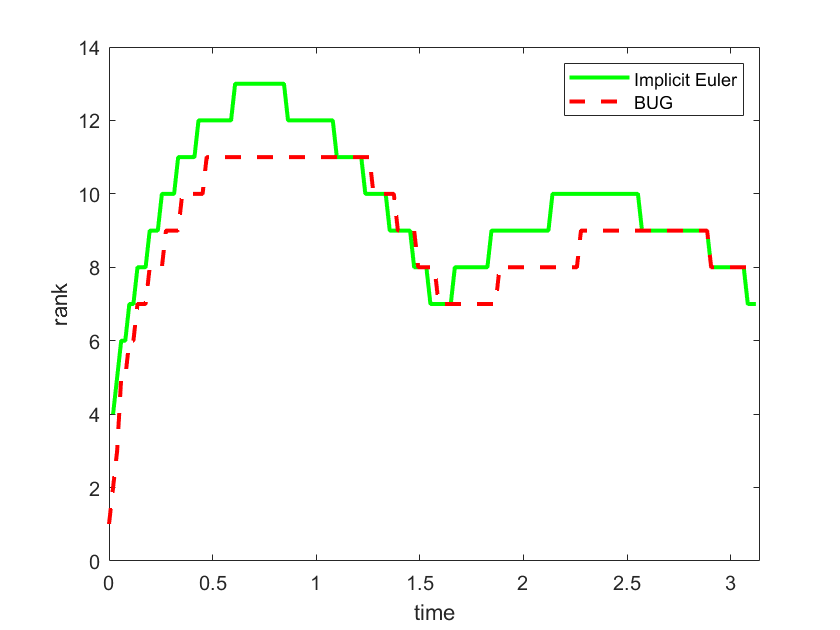
\includegraphics[width=0.5\linewidth]{rank-time.png}
        \caption{XXX}
    \end{figure}
\end{frame}

\begin{frame}{Figures}
    \begin{figure}[htbp]
        \centering
        \begin{subfigure}[b]{0.45\textwidth}
            \centering
            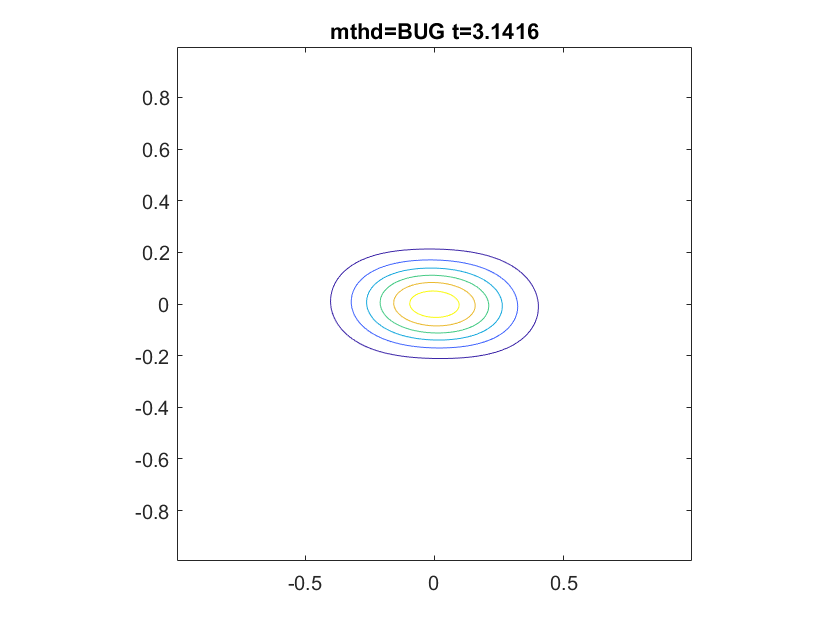
\includegraphics[width=\textwidth]{bug.png}
            \caption{XXX}\label{fig:subfig-a}
        \end{subfigure}
        \begin{subfigure}[b]{0.45\textwidth}
            \centering
            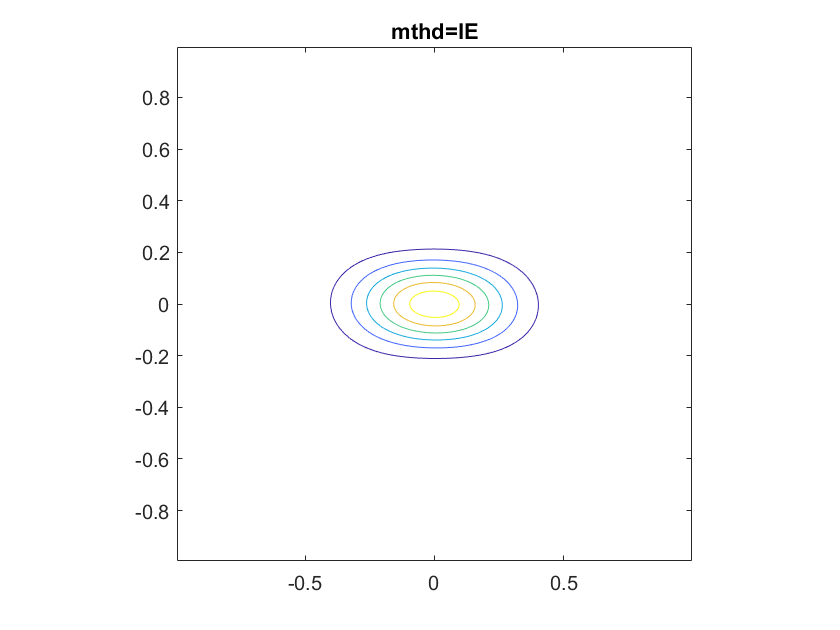
\includegraphics[width=\textwidth]{ie.png}
            \caption{XXX}\label{fig:subfig-b}
        \end{subfigure}
        \caption{XXX}\label{fig:example}
    \end{figure}
\end{frame}


\begin{frame}{Figure + Columns}
    \begin{columns}
        \column{0.6\textwidth}
        \begin{figure}
            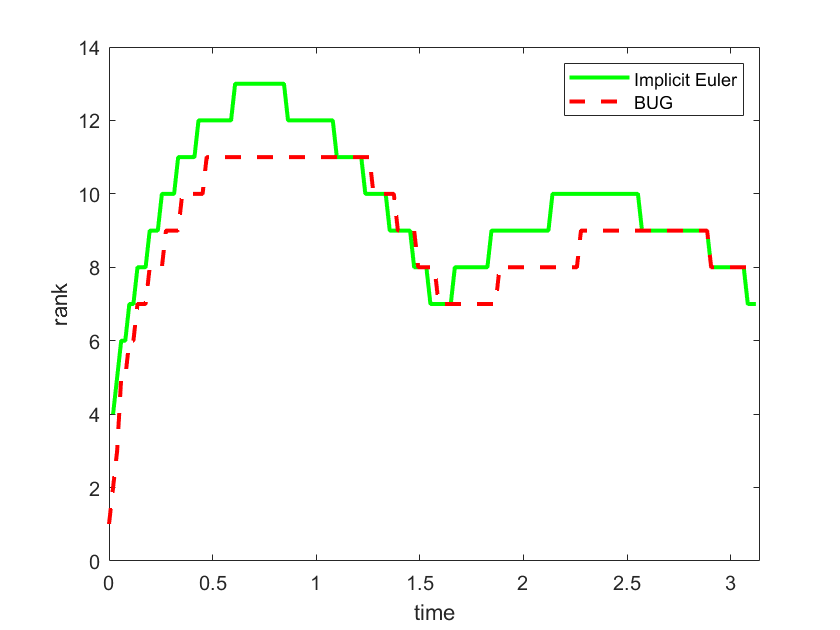
\includegraphics[width=0.8\linewidth]{rank-time.png}
            \caption{XXX}
        \end{figure}
        \column{0.4\textwidth}
        This is column one with 0.4 text width.
    \end{columns}
\end{frame}

\subsection{Algorithm \& Code}

\begin{frame}{Algorithm}
    \begin{algorithm}[H]
        \caption{Euclid's algorithm}
        \KwData{Two nonnegative integers $a$ and $b$}
        \KwResult{Their greatest common divisor $d = \gcd(a, b)$}
        \While{$b \neq 0$}{
            $r \leftarrow a \bmod b$\;
            $a \leftarrow b$\;
            $b \leftarrow r$\;
        }
        $d \leftarrow a$\;
    \end{algorithm}

\end{frame}

\begin{frame}[fragile]{Code}

    \begin{lstlisting}[language=c++]
#include <iostream>

int main() {
    std::cout << "Hello, world!" << std::endl;
    return 0;
}
\end{lstlisting}
    \begin{lstlisting}[language=python]
def greet(name):
    print(f"Hello, {name}!")

greet("John")
\end{lstlisting}

\end{frame}


\section{Conclusion}

\begin{frame}{Conclusion \& Future work}
    \begin{itemize}
        \item This is the conclusion
              \medskip
        \item This is the future work
    \end{itemize}
\end{frame}

\begin{frame}[plain]
    \vspace{0.3\textheight}
    \Huge{\centerline{\color{simplebeamercolor}\textbf{Thank You!}}}
\end{frame}

\end{document}
